%%%%%%%%%%%%%%%%%%%%%%% file template.tex %%%%%%%%%%%%%%%%%%%%%%%%%
%
% This is a general template file for the LaTeX package SVJour3
% for Springer journals.          Springer Heidelberg 2010/09/16
%
% Copy it to a new file with a new name and use it as the basis
% for your article. Delete % signs as needed.
%
% This template includes a few options for different layouts and
% content for various journals. Please consult a previous issue of
% your journal as needed.
%
%%%%%%%%%%%%%%%%%%%%%%%%%%%%%%%%%%%%%%%%%%%%%%%%%%%%%%%%%%%%%%%%%%%
%
% First comes an example EPS file -- just ignore it and
% proceed on the \documentclass line
% your LaTeX will extract the file if required
\begin{filecontents*}{example.eps}
%!PS-Adobe-3.0 EPSF-3.0
%%BoundingBox: 19 19 221 221
%%CreationDate: Mon Sep 29 1997
%%Creator: programmed by hand (JK)
%%EndComments
gsave
newpath
  20 20 moveto
  20 220 lineto
  220 220 lineto
  220 20 lineto
closepath
2 setlinewidth
gsave
  .4 setgray fill
grestore
stroke
grestore
\end{filecontents*}
%
\RequirePackage{fix-cm}
%
\documentclass{svjour3}                     % onecolumn (standard format)
%\documentclass[smallcondensed]{svjour3}     % onecolumn (ditto)
% \documentclass[smallextended]{svjour3}       % onecolumn (second format)
%\documentclass[twocolumn]{svjour3}          % twocolumn
%
\smartqed  % flush right qed marks, e.g. at end of proof
%
\usepackage{graphicx}
\usepackage{enumitem}
\usepackage{float}
% \usepackage{caption}
\usepackage{subfig}
\usepackage{cite}
\usepackage{url}
\usepackage{spreadtab}
\usepackage{algorithm,algorithmic}
\usepackage{amsmath}
\usepackage[numbers]{natbib}

\DeclareMathOperator*{\argmin}{argmin} % thin space, limits underneath in displays
\DeclareMathOperator*{\myint}{int} %
%
% \usepackage{mathptmx}      % use Times fonts if available on your TeX system
%
% insert here the call for the packages your document requires
%\usepackage{latexsym}
% etc.
%
% please place your own definitions here and don't use \def but
% \newcommand{}{}
%
% Insert the name of "your journal" with
% \journalname{myjournal}
%
\begin{document}

\title{Flexible needle and patient tracking using fractional scanning for reduced dose in interventional CT procedures
%\thanks{Grants or other notes
%about the article that should go on the front page should be
%placed here. General acknowledgments should be placed at the end of the article.}
\thanks{Research supported by Kamin grant 57706, Office of the Chief Scientist, Ministry of Trade and Industry, Israel. We thank Eyal Lin and Ronen Shter of GE Healthcare Israel for the CT scans and for their valuable assistance.}% <-this % stops a space
% \thanks{G. Medan and L. Joskowicz are with the CASMIP Laboratory, School of Computer Science and Engineering, The Hebrew University of Jerusalem, Israel (josko@cs.huji.ac.il).}%
}
% \subtitle{Do you have a subtitle?\\ If so, write it here}

\titlerunning{Reduced dose flexible needle and patient tracking}        % if too long for running head

\author{Guy Medan         \and
        Leo Joskowicz %etc.
}

%\authorrunning{Short form of author list} % if too long for running head

\institute{
  L. Joskowicz, G. Medan \at
  CASMIP  Laboratory\\
  School  of  Computer  Science  and  Engineering\\
  The  Hebrew  University of Jerusalem, Israel\\
  \email{josko/gmedan@cs.huji.ac.il}           %  \\
%             \emph{Present address:} of F. Author  %  if needed
}

% \date{Received: date / Accepted: date}
% The correct dates will be entered by the editor


\maketitle

\begin{abstract}
We present a new method for flexible needle and patient localization in interventional CT procedures based on fractional CT scanning.
Our method accurately localizes the trajectory of a flexible needle to which a spherical marker is attached at a known distance from the tip with respect to a baseline scan of patient in the CT scanner coordinate frame. 
The localization is achieved with a significantly lower dose compared to a full scan using sparse view angle sampling and without reconstructing the CT image of the repeat scan.
Our method starts by performing rigid registration between the patient and the baseline scan in Radon space computed from the sparse projection data.  It then computes projection difference images in which the needle and the spherical marker appear as prominent features. Their 3D spatial locations are then automatically extracted from these 2D projection images to trace the needle trajectory. To validate our method, we conducted registration and needle trajectory localization experiments in seven abdomen phantom scans using two types of flexible needles. Our experimental results yield a mean needle trajectory localization error of 0.7 $\pm$ 0.2mm and a mean
tip localization error of 2.4 $\pm$ 0.9 mm with a x7.5 radiation dose reduction with respect to a full scan. The dose reduction enables more frequent needle trajectory localization during the needle insertion for a similar total dose, or a reduced total dose for the same localization frequency.
\keywords{
interventional CT \and 
fractional CT scanning \and 
reduced dose CT scanning \and 
flexible needle tracking \and
Radon space registration 
}
\end{abstract}

\section*{Introduction}

Image guided minimally invasive techniques have become commonplace for interventional procedures such as biopsies and aspirations.
In these procedures, a flexible needle is inserted under image guidance towards a target, either manually or using robotic actuators. Repeated imaging is required during insertion to ensure that the needle is advancing in the desired direction and to correct the insertion path as required. Localization errors of a few millimeters in the needle insertion trajectory and its final placement can lead to misdiagnosis, repeated insertion attempts, and failed treatment.

CT guidance is often used in interventional radiology procedures to help the surgeon guide the needle towards the desired target. CT imaging is unique in that it provides real-time high resolution axial in-plane and volumetric images of the patient and the needle. However,
CT-guided interventions has several limitations and drawbacks.
The intervention protocol typically requires the needle to be aligned with the axial plane of imaging as it is being inserted \cite{gupta2014ct}, which requires careful positioning of the patient to allow access to the target. In addition, the presence of the needle in the scanned volume introduces imaging artifacts caused by beam hardening and scatter \cite{boas2012ctartifacts}, which can obscure important anatomical structures near the needle tip. Finally, the patient's cumulative exposure to ionizing X-ray radiation may increase the risk of cancer \cite{mettler2000ct, chodick2007excess}, which is exacerbated in interventional CT due to the number of repeat scans acquired during the procedure.

Other imaging modalities used for interventional procedures include ultrasound, X-ray fluoroscopy and cone-beam CT.
Ultrasound is a cost effective imaging solution. However, it only provides 2D cross sectional images with limited resolution and a low signal-to-noise ratio (SNR) \cite{sheafor2000comparison}. Although 3D/4D Ultrasound imaging is becoming more available in recent years, 
its use si still limited in clinical practice.
X-ray fluoroscopy offers improved spatial resolution, but is not suitable for procedures that require axial views or when complex anatomical relationships must be characterized in 3D during the intervention.
Flat-panel cone-beam CT is a relatively new technology increasingly used in interventional radiology. However it has longer scan times and increased radiation scatter, resulting in increased artifacts compared to multi-detector CT \cite{orth2008cbct}. Recent advances have reduced scan times to 5-20 seconds, with a x2-3 radiation dose reduction \cite{dynact}.

Dose reduction techniques for CT mainly focus on achieving a good quality of reconstruction for a single, standalone scan acquisition. The most common radiation dose reduction technique is scanning with a lower tube current. This lowers the scanning SNR, which results in noise, lowered imaging contrast and resolution, and  introduces artifacts. Several methods have been developed to address these problems, including image denoising \cite{manduca2009projection} and image reconstruction with statistical noise models  \cite{zhang2016statistical,kim2015sparseview,niu2014sparse,liu2014total}. The radiation dose is typically x2-3 times that of a full scan. 

We have recently introduced a novel approach to CT radiation dose reduction in situations in which a full baseline CT scan is available, as is usually the case in interventional CT procedures \cite{medan2017sparse, medan2017reduced}. In our approach, subsequent full dose scanning is replaced by fractional scanning, which consists of the selective acquisition of a sparse set of projection views. Fractional scanning reduces the radiation dose by modulating the current to the source of X-rays during its rotation. By exploiting the projection space raw data, registration with the baseline scan and localization of the needle in the repeat scan can be achieved without reconstruction of the repeat scan image. This technique yields a x9-20 radiation dose reduction.

%Dose reduction for physician
The reduction of dose has implications for medical staff as well as patients, since the time spent by physicians, nurses and technologists throughout their careers in the intervention suite necessarily involves exposure to ionizing radiation. While protection equipment is used by medical professionals, the cumulative exposure has been linked to an increased risk of cataracts and cancer \cite{miller2010occupational, sarti2012low}. In interventional CT, it is important to develop methods allowing dose reduction for slightly different concerns, such as excessive dose to the radiologist's hands \cite{stoeckelhuber2005radiation}.

\section*{Previous work}
Various methods have been recently developed to achieve accurate needle insertion by robotic actuators. These works focus on the mechanical modelling of the robotic system, the patient anatomy, and the needle trajectory planning, with less attention to needle localization from imaging modalities.
Wu et al. \cite{wu2013automatic} and Engh et al. \cite{engh2010percutaneous} describe implementations of a bevel-tip needle steering method using duty-cycle spinning of the needle that relies on the needle bending tendency due to asymmetry. Such systems model the needle-tissue interaction to execute a control sequence to follow a pre-planned trajectory. Image-based feedback is mentioned as a means to allow corrections of the control sequence mid-insertion by adjusting the planned trajectory based on the actual needle trajectory.
Ben-David et al. \cite{ben2018robotic} describe a robotic system for flexible needle insertion under CT guidance. A dual guiding mechanism is composed of a driver that advances the needle while a positioning unit steers it during the insertion. A pre-planned 3D trajectory is executed and corrected during the insertion based on full repeated CT scans.
Earlier work by Glozman et al. \cite{glozman2007image} describes robotic flexible needle steering and a needle-tissue mechanical interaction model. The steering feedback is based on 2D in-plane imaging of the needle.

Most works in needle localization from medical images use ultrasound as the imaging modality. A robotically positioned 2D transducer perpendicular to the needle tip is presented in Vrooijink et al. \cite{vrooijink2013real}. In this system, needle-induced image artifacts are used to localize the needle tip in the imaged plane. The ultrasound transducer is continuously re-positioned to maintain its orientation relative to the needle tip. An approach combining both ultrasound and CT fluoroscopy is presented in \cite{marinetto2017integration}. In this approach, a free-hand ultrasound probe and a fluroscopic C-arm are registered using an external optical tracker to produce a fused image in which the needle can be tracked.

Several works describe specific methods to localize the needle trajectory in reconstructed CT images. 
In previous work by the authors \cite{medan2017reduced}, localization of a straight rigid needle is addressed. The needle path is found by an intersection of planes in 3D space computed from 2D projection images. 
Hou et al. \cite{huo2015shape} reconstruct the bevel-tip flexible needle trajectory from full CT slices by localizing points at which the needle intersects slice planes, and fitting a fourth-order polynomial to the collection of 3D points.
Yaniv et al. \cite{yaniv2010needle} describe a system in which embedded electromagnetic fiducials are used for needle tracking under CT guidance. Operator input is required to identify the needle tip in a full CT scan taken in-situ. These methods rely on the acquisition of a full repeat CT scan and on the reconstruction of the image for each localization of the needle. This approach carries the associated cost in radiation dose for the patient. 

In a different clinical application, Cong et al.  \cite{cong2015quantitative} show that the 3D structure of coronary arteries can be reconstructed from a few X-ray angiography views using forward projection of an evolving parametric 3D model into 2D projections and updating the model based on the projection images. This method may be applicable to track the location of a needle and patient anatomy, although it has not been tried yet. 

\section*{Method}

We describe next a new method for flexible needle and patient localization in interventional CT procedures based on fractional CT scanning. We begin by computing a sinogram-space rigid registration of the patient position in the CT scanner coordinate frame between a baseline scan without a needle, and a repeat scan with a needle introduced. The repeat scan is performed by sampling sparsely in the view angle domain (fractional scanning) and without reconstructing the CT image, while the baseline scan is assumed to be a full scan (sampled densely in the view angle domain). We use projection difference images (shown in Fig. \ref{proj_diff_fig}), which are calculated by subtracting registered reprojected baseline scan images from the sparse set of repeat projection images. These highlight the differences between scans, which in our case is assumed to be the needle. The needle trajectory is then traced in 3D space using only the projection difference images. The stages of our method are:
\begin{enumerate}
\item \textit{Fractional scanning}. A fractional repeat scan is obtained with the needle in place. The full baseline scan and fractional repeat scan are registered using our sinogram space rigid registration method \cite{medan2017sparse}.
\item \textit{Projection difference}. Using the obtained rigid registration, the projection difference images are computed by applying the rigid transformation to the baseline scan volume, forward projection, and subtracting from corresponding repeat scan projection images. The images are then post-processed by computing the gradient intensity image and normalizing by the local mean gradient intensity value, to obtain an image in which the features of the projection difference have intensities on the same order of magnitude.
\item \textit{Spherical marker localization}. The 3D localization of the spherical marker attached to the needle at a known distance from the tip is computed using the projection difference images.
\item \textit{Incremental needle trajectory tracing}. The needle trajectory is incrementally computed in 3D space using the projection difference images, starting from the center of the marker obtained in the previous stage. 
\item \textit{Display/feedback}. The current location of the needle with respect to the baseline scan 3D image is displayed and/or used as feedback for gradually driving the needle towards the target.
\end{enumerate}
Steps 1-5 are repeated each time the needle is gradually inserted during the intervention, until the tip localization shows the desired target structure in the patient's anatomy is reached. Optionally, full CT scans for image reconstruction can be acquired during the procedure as needed. Our method uses the same sparse projection sampling pattern both for registration and for needle localization, thereby avoiding additional scanning and image reconstruction. In this case, the radiation dose is a fraction of that required in image based methods. This allows frequent needle insertion and localization for feedback and accuracy without excessive radiation dose.

The rest of this section is organized as follows.
Section \ref{markerloc} summarizes the step for localizing the spherical marker in 3D space.
Section \ref{inctracing} provides a detailed description of the incremental 3D curve tracing algorithm.

\subsection{Marker localization} \label{markerloc}
The 3D center of the spherical marker is localized in three stages:
\begin{enumerate}
    \item 
    {
    The 2D centers of the projected spherical marker are approximately localized in each of the $K$ projection difference images by correlating the difference projection image with a circular pattern. 
    }
    \item 
    {
    The location of the 2D projected marker center in each projection difference image is refined by optimizing a cost function that  takes into account the image gradients of the marker's surface:
    \begin{equation}
        c_j = \argmin_{c \in \rm I\!R^2}{
        \iint_{\lvert \, \lvert\lvert x-c \rvert\rvert - R \rvert < \epsilon}
        {\nabla h_j(x) \cdot \hat{r}_c} \, \mathrm{d}x}
    \end{equation}
    where $h_j(x)$ is the projection difference image for view $j$, $R$ is the known radius of the marker, and $\epsilon$ is a small distance parameter set to the physical size of one detector pixel, so that the gradient of the projection difference image is best aligned with the radial direction $\frac{(x-c)}{ \\\lvert\lvert x-c \rvert\rvert}$ inside a spherical shell of radius R and thickness $2\epsilon$.
    }
    \item
    {
    The 3D location of the marker center is computed by solving an inverse problem using the known projection geometry of the CT and the localized marker centers described by transformation matrices $P_j$. The solution of the set of projection equations $\{P_j s = c_j\}_{j=1}^K$  yields the 3D marker center location $s$.
    }
\end{enumerate}



\subsection{Incremental trajectory tracing} \label{inctracing}

The trajectory of the needle in 3D space is estimated by incrementally establishing a series of equidistant landmark points along the trajectory of the needle in 3D space $p_1, p_2, ..., p_i$. These landmark points are then fitted to cubic B\'ezier curve $C_i$  that traces the curvilinear shape of the needle from the center of the spherical marker toward the last point $p_i$, where $i$ is the number of landmark points. The points fitting to the Bezier curve is obtained with the method by Khan \cite{khan2007approximation}. The method computes the cubic B\'ezier curve in 3D space such that the squared-sum-distance of the landmark points from the curve is minimized. The sequence of landmark points is initialized with four co-linear and equidistant points starting from the marker center $p_1=s$. with successive distance $\Gamma$ along an initial direction determined by optimization of a cost function detailed in the following paragraph. The  parameter  $\Gamma$ is a fixed parameter for segment length. The minimal number of landmark points required to calculate a cubic B\'ezier curve is four. 

%\begin{enumerate}
 %\item Starting from the center of the spherical marker, the initial direction of the first needle segment is determined in 3D space using its 2D projections onto the projection difference images, by optimizing a cost function which is designed to attain a minimum when the projection difference images contain line segment in the projected direction. Four control points are placed at regular intervals along the initial segment.
 %\item Starting from the end of the previous segment, the next segment direction is determined in 3D space in a similar manner, and one control point is placed at the new segment end.
 %\item The process is repeated and the accumulated control points are used to evaluate a B\'ezier curve in 3D space such that the sum squared distances of the control points from the curve is minimized.
 %\item Once the length of the evaluated curve exceeds the known distance between the tip and the center of the spherical marker, the last segment is shortened accordingly, with the last point representing the tip localization.
%\end{enumerate}

\begin{table}
\hline
\begin{algorithmic}
  \STATE
  \STATE INPUT: projection difference image
  \STATE $s\leftarrow$ localize spherical marker
  \STATE $\hat{n}_1 \leftarrow$ estimate initial needle direction
  \STATE $p_1, p_2, p_3, p_4 \leftarrow$ initialize from $s$ along $\hat{n}_1$
  \STATE $L\leftarrow 3\Gamma$ 
  \STATE $i\leftarrow 4$
  \WHILE{$L < L_{marker,tip}$}
    \STATE $\hat{n}_{i} \leftarrow$ estimate needle direction starting from $p_i$
    \STATE $p_{i+1} \leftarrow p_i + \Gamma \hat{n}_{i}$
    \STATE $C_{i+1}\leftarrow$ fit cubic B\'ezier curve to $p_1, ..., p_{i+1}$
    \STATE $L\leftarrow length(C_{i+1})$ 
    \STATE $i\leftarrow i+1$
  \ENDWHILE
  \STATE adjust $p_i$ such that $length(C_i) = L_{marker,tip}$
  \STATE
\end{algorithmic}
\hline
\caption{Needle trajectory tracing algorithm.}
\label{algo}
\end{table}

Table \ref{algo} presents the algorithm. 
In each iteration a new point $p_{i+1}(\hat{n}) = p_i + \Gamma \hat{n}$ is sought and $\hat{n}$ is a direction to be determined via optimization of a cost function detailed below.
A 3D curve $C_{i+1}[\hat{n}]$ is fitted to the landmark points $p_1, p_2, ..., p_i, p_{i+1}(\hat{n})$, and projected onto each of the $K$ view angles projection difference images to obtain projected curves $P_j C_{i+1}[\hat{n}] = c_{i+1}^j[\hat{n}]$ where $j=1,...,K$ is the view angle index and $P_j$ is the projection operator for view $j$.
The direction $\hat{n}$ is obtained by optimizing a cost function designed to attain a minimum when the projection of the curve $C_{i+1}$ onto the set of projection difference images follows the needle trajectory traced in the images:
\[ \Psi_i(\theta, \phi) = -\sum_{j=1}^K{\int_{r \in c_{i+1}^j[\hat{n}(\theta, \phi)]} {I_j(r)dl}} \]
where $ \theta, \phi$ are spherical coordinates, $ \hat{n}(\theta, \phi) $ is the conversion from spherical coordinates to unit vector $ \hat{n} $, and $r$ is the 2D coordinate along the projected trajectory $c_{i+1}^j[\hat{n}]$ in projection difference image $I_j$. The projection difference image is signed, therefore pixels with large positive values correspond to coordinates in which the needle passes in the repeat scan but is absent in the baseline, and the needle segment corresponds to a high intensity section of the difference image.
Accordingly, the orientation of the $i$-th segment is obtained as $(\theta_i^*, \phi_i^*) = \textsf{argmin}_{\theta, \phi} \Psi_i ( \theta, \phi)$. Then, a new landmark point $p_{i+1}$ is added to the series of established landmark points $p_1, p_2, ..., p_i$ using the relation:
$$ p_{i+1} = p_i + \Gamma \hat{n}(\theta_i^*, \phi_i^*) $$

The incremental process is stopped once the length of the 3D curve $C_{i+1}$ exceeds the known distance between the marker and needle tip. Then, the tip position is determined by trimming the last segment so that the overall length of the curve is equal to the known marker-tip distance.

\section*{Results}

To demonstrate our method we conducted an experiment consisting of flexible needles inserted into an abdomen phantom (CIRS model 57 Triple Modality 3D Abdominal Phantom) and scanned using GE Discovery CT750HD scanner at GE Healthcare Haifa (see Fig. \ref{long_needle_fig}). The needles used were: a long 16 gauge (1.65mm outer diameter) needle, and short 22 gauge (0.72mm outer diameter) needle. For the long needle, the marker center was fixed at 235mm from the tip, and for the short needle at 135mm (figures \ref{long_needle_fig} and \ref{short_needle_fig} respectively).
The reconstructed image size is 800$\times$800$\times$144 voxels, with spatial resolution of 0.58$\times$0.58$\times$1.25 mm$^3$. The detector array consists of 885 elements scanned at 984 views at regular intervals in the range [0$^{\circ}$ , 360$^{\circ}$), where four slices were acquired in each full revolution. The data was re-binned from fan-beam to parallel rays representation of the projections.

At first a scan of the empty scanner bed was performed so that its sinogram can be subtracted from the following scans (this is done since the scanner bed does not undergo the same rigid movement as the phantom). Then, a full (i.e. dense sampling of view angles) baseline scan of the phantom was acquired, without the needle present. At each subsequent scan, the needle with attached spherical marker was inserted at a different location or different depth, the entire phantom was rotated by up to 5$^\circ$ about an arbitrary axis and/or translated by up to 5cm, and a full scan was acquired again. Sparse scanning was simulated by allowing the algorithm to access only a small subset of view angles.


% \begin{figure}[b]
% \centering
% 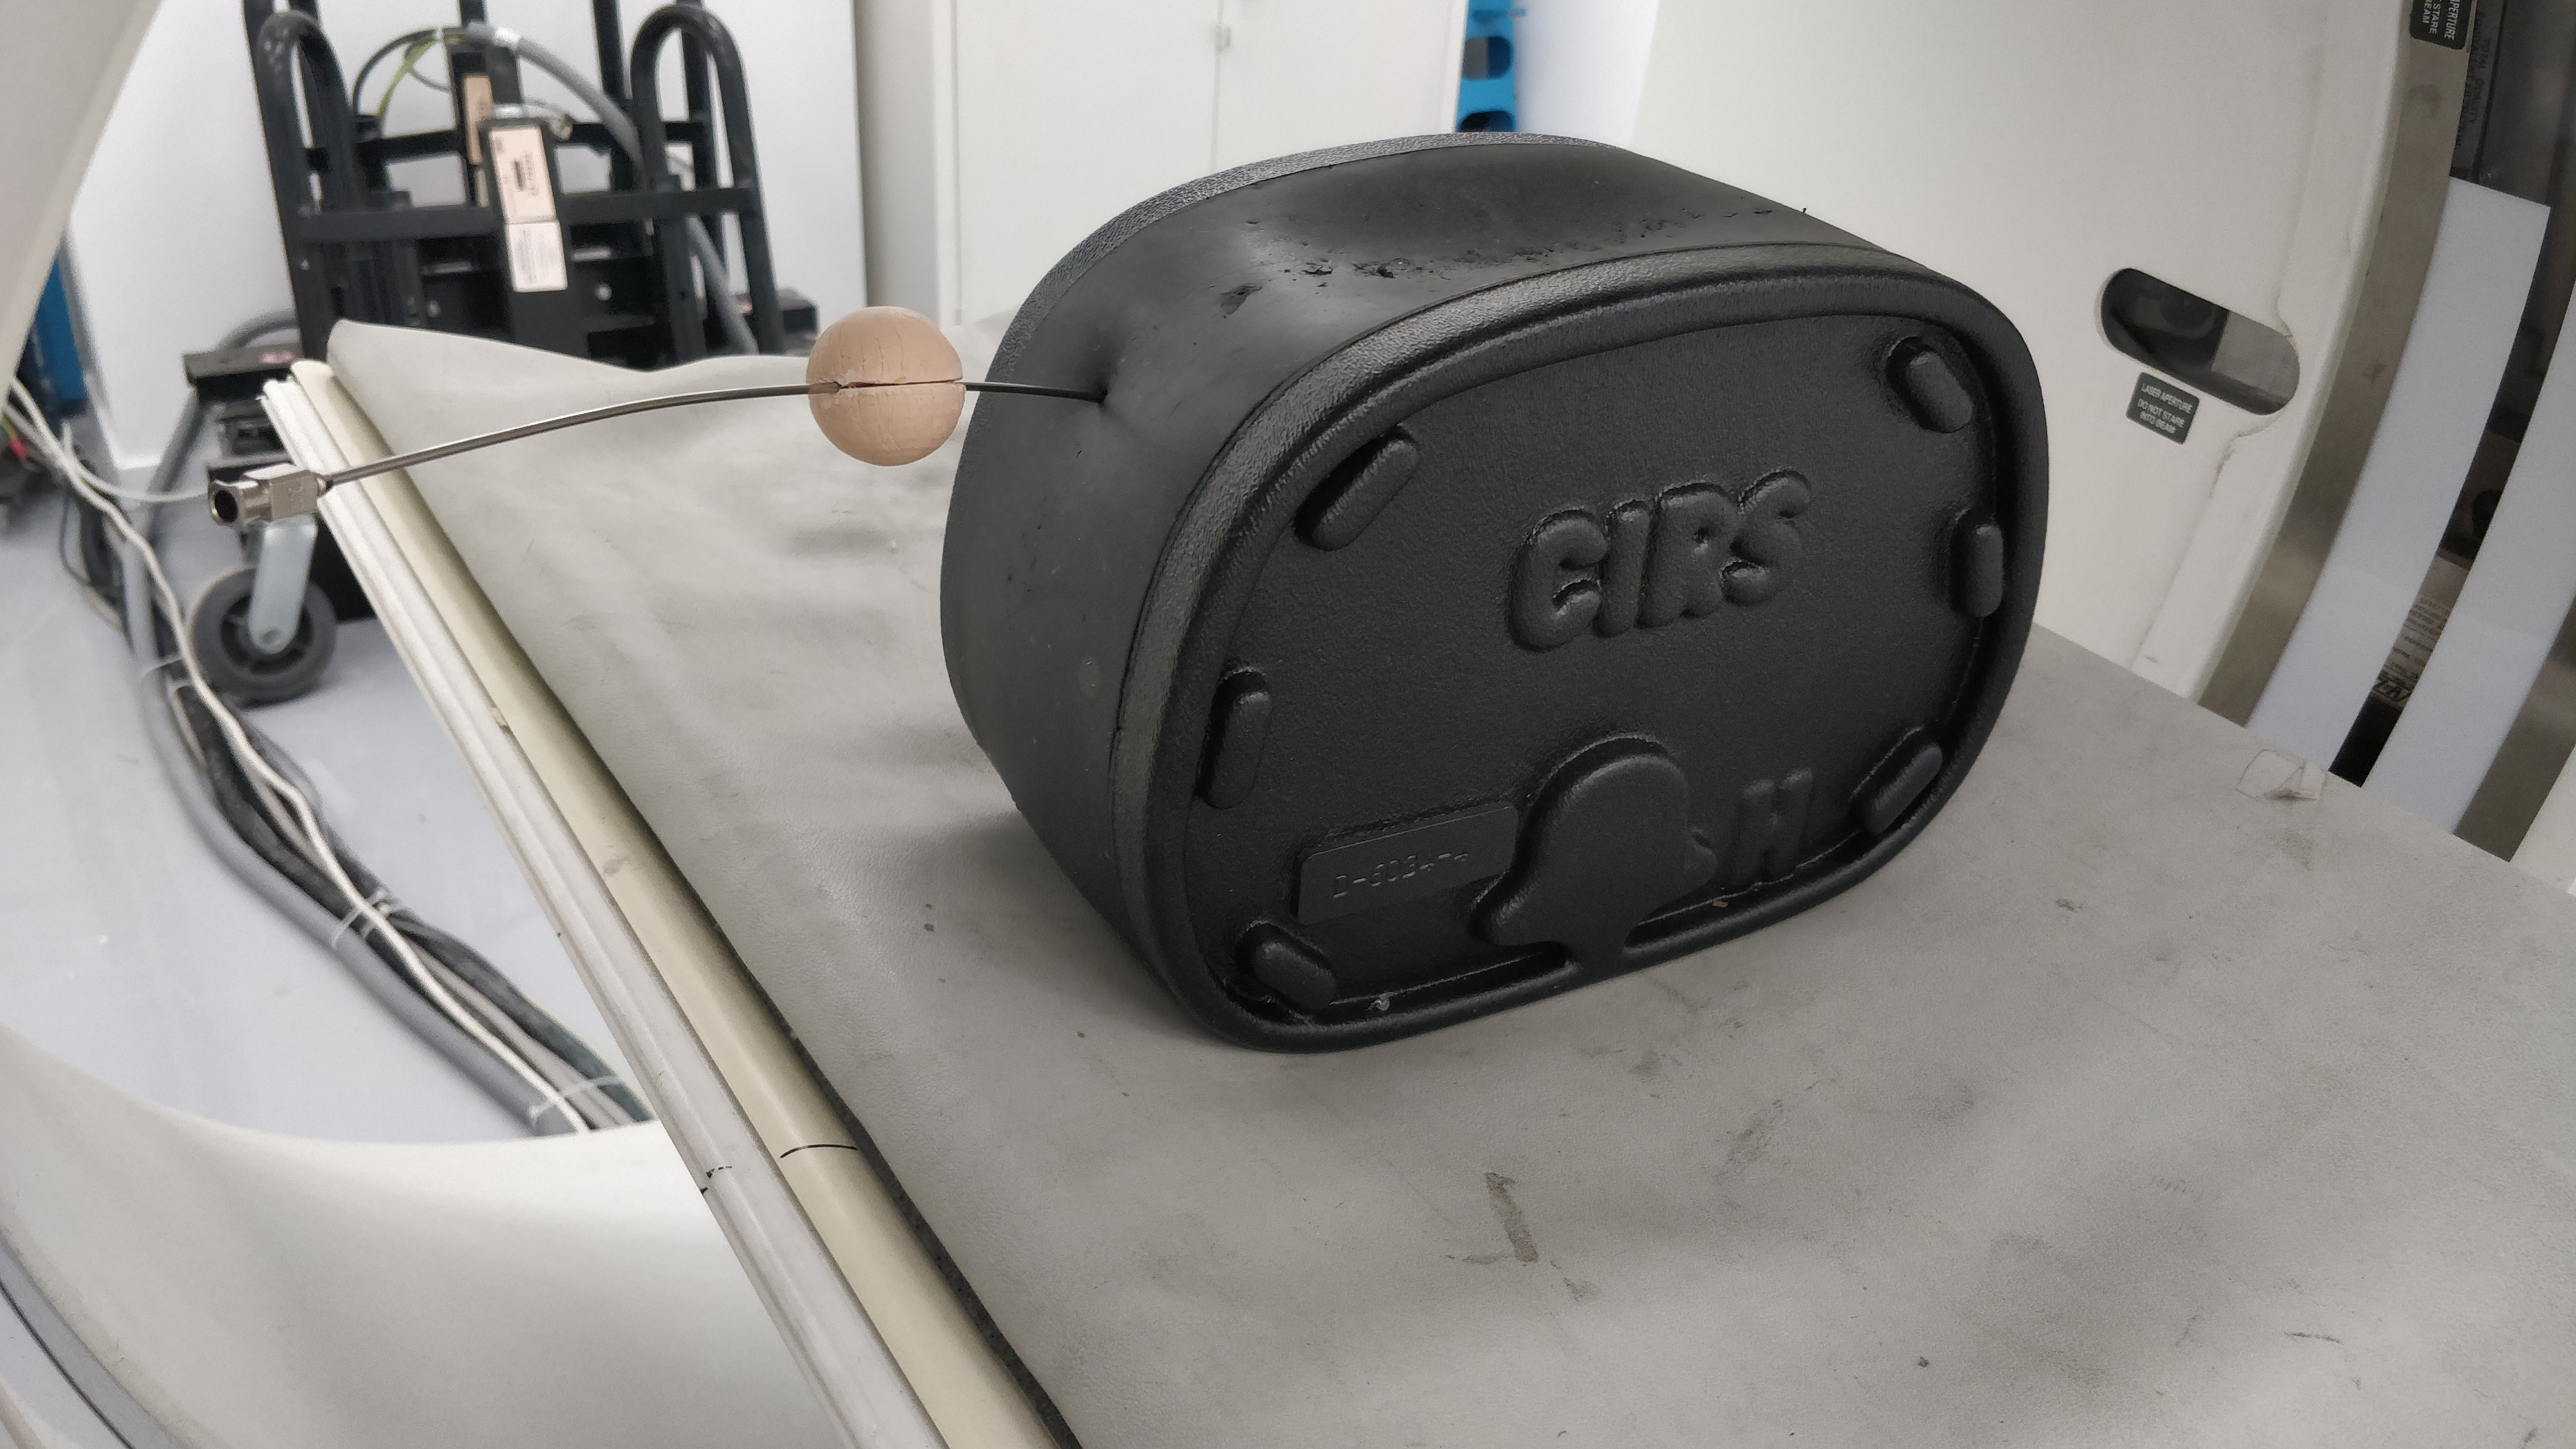
\includegraphics[width=8cm]{long_needle_phantom.jpg}
% \caption{\small{Photograph of the long flexible needle with spherical marker inserted into abdomen phantom lying on the CT scanner bed.}}
% \label{long_needle_fig}
% \end{figure}

% \begin{figure}[t]
% \centering
% 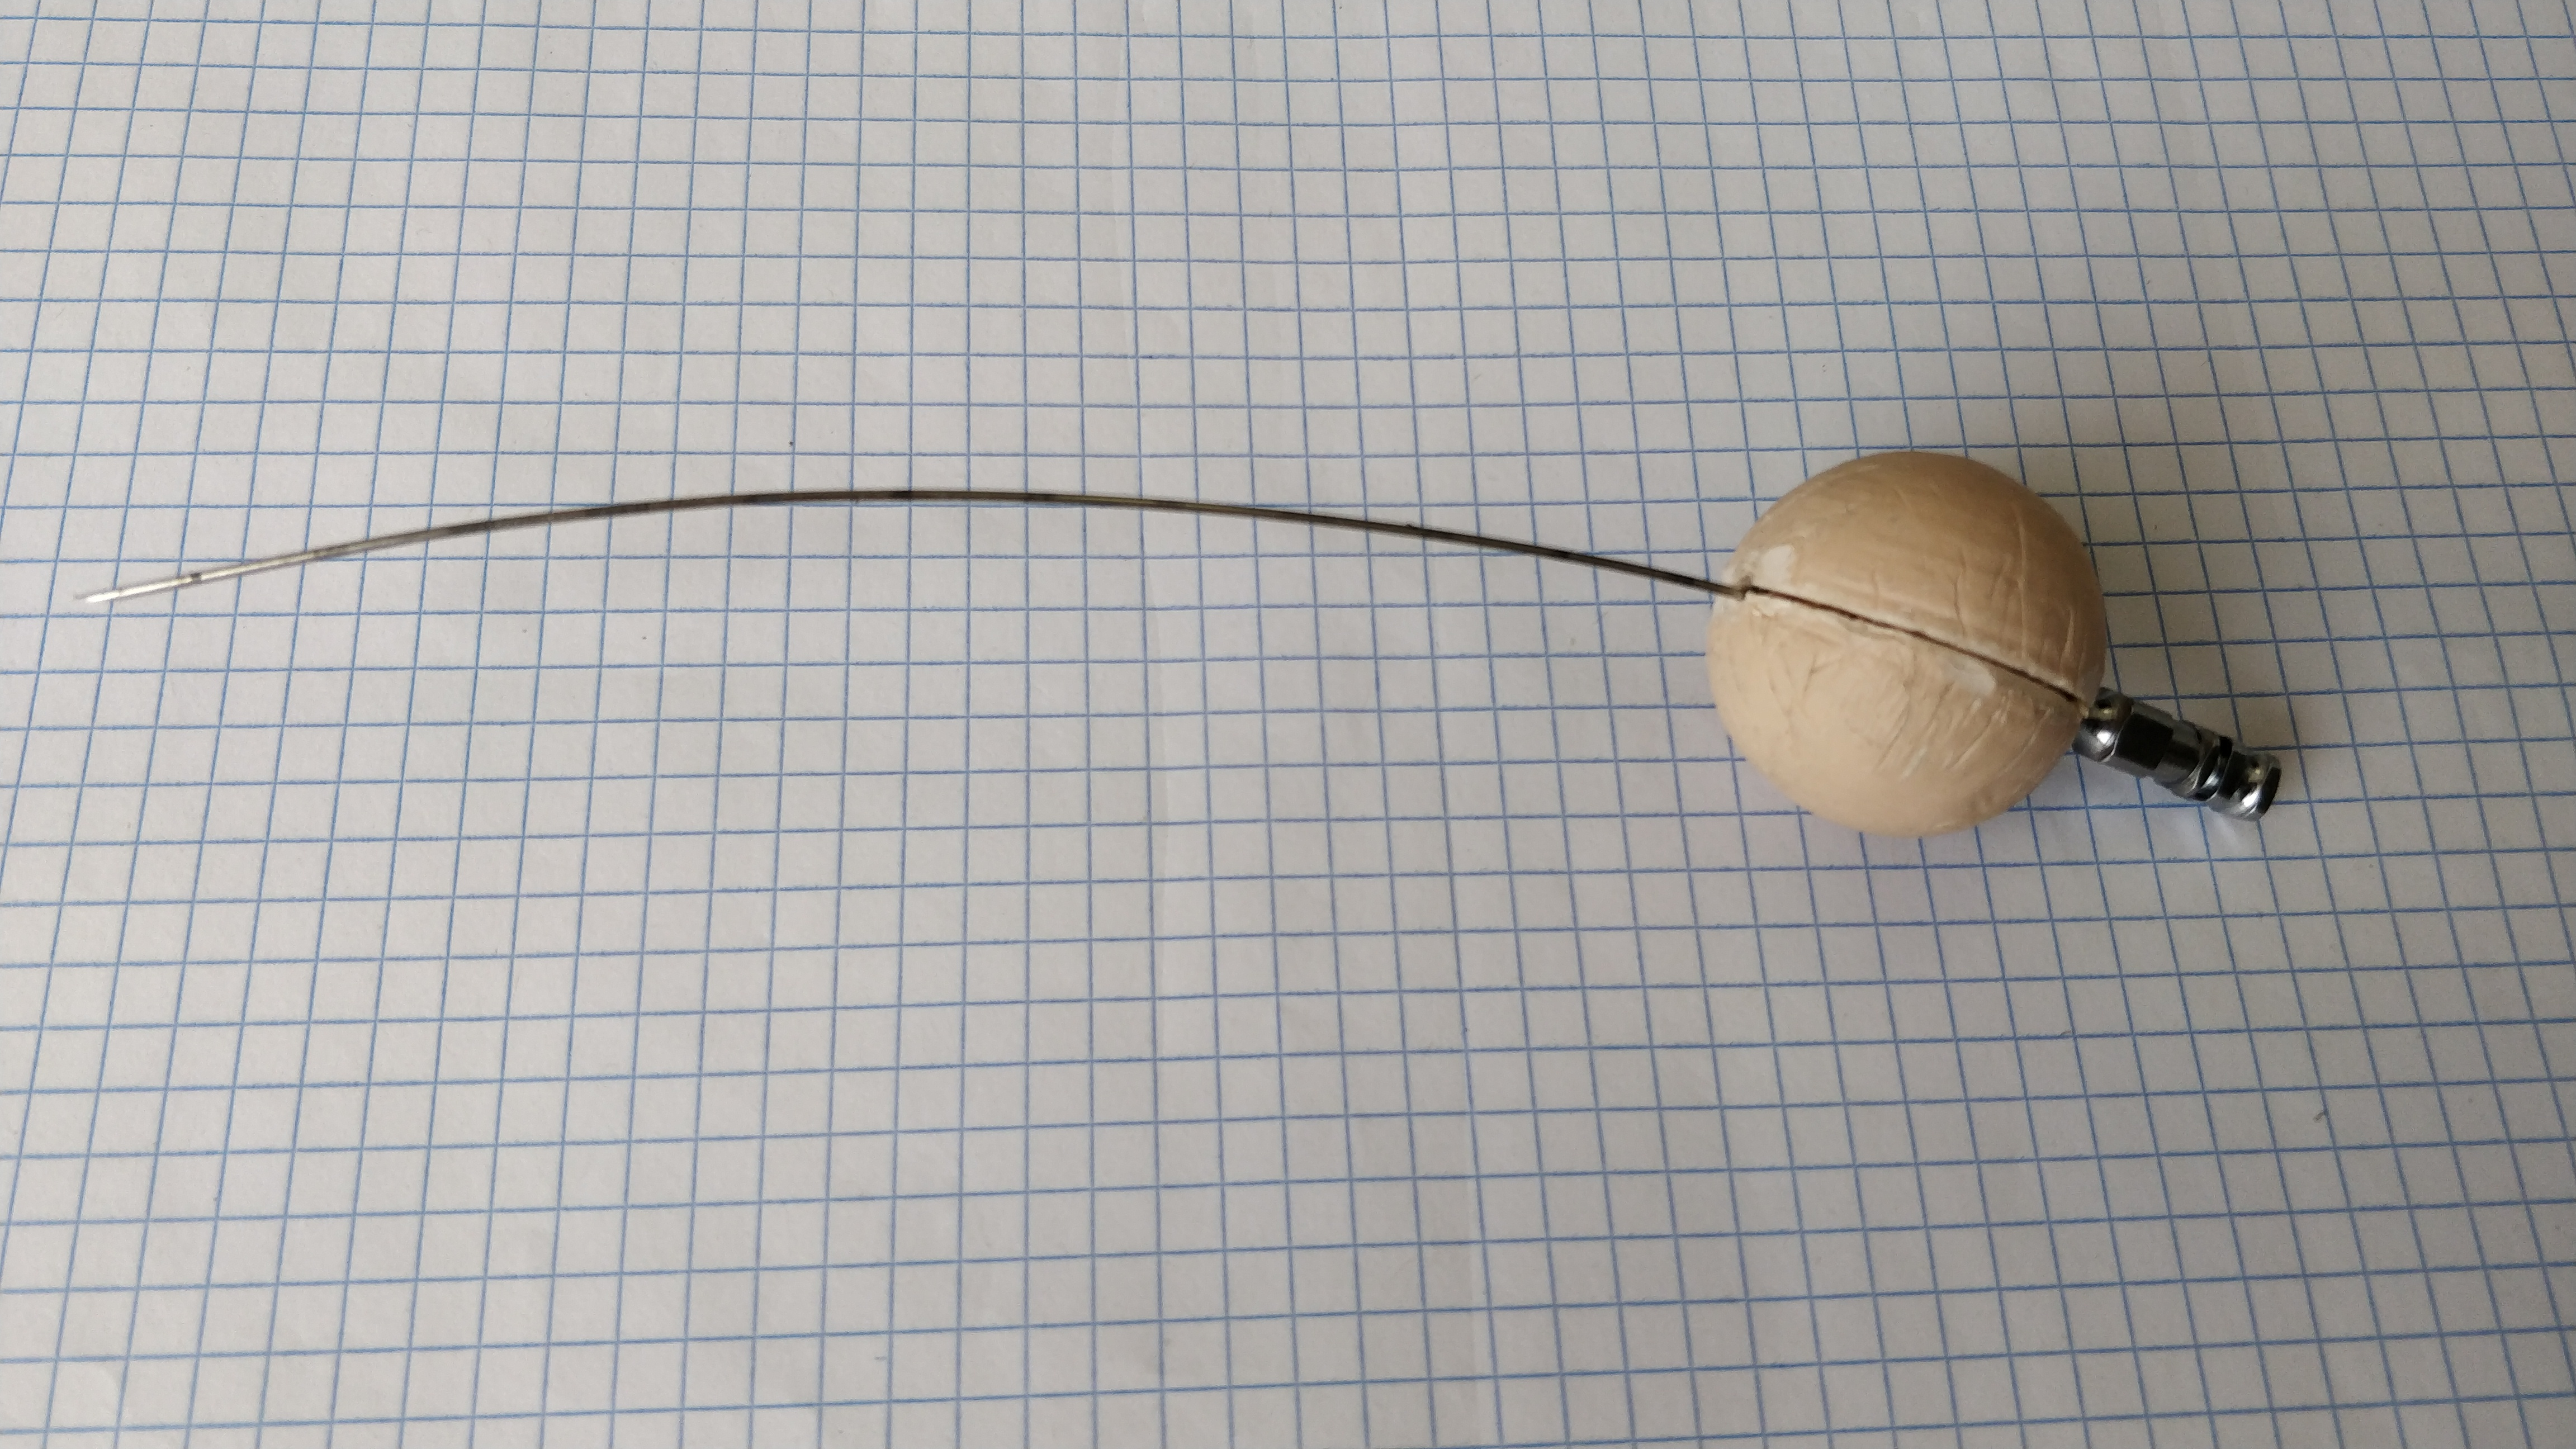
\includegraphics[width=8cm]{short_needle.jpg}
% \caption{\small{Photograph of the short flexible needle with spherical marker attached at 135mm from the tip.}}
% \label{short_needle_fig}
% \end{figure}


\begin{figure*}[t]
  \centering
  \subfloat[]{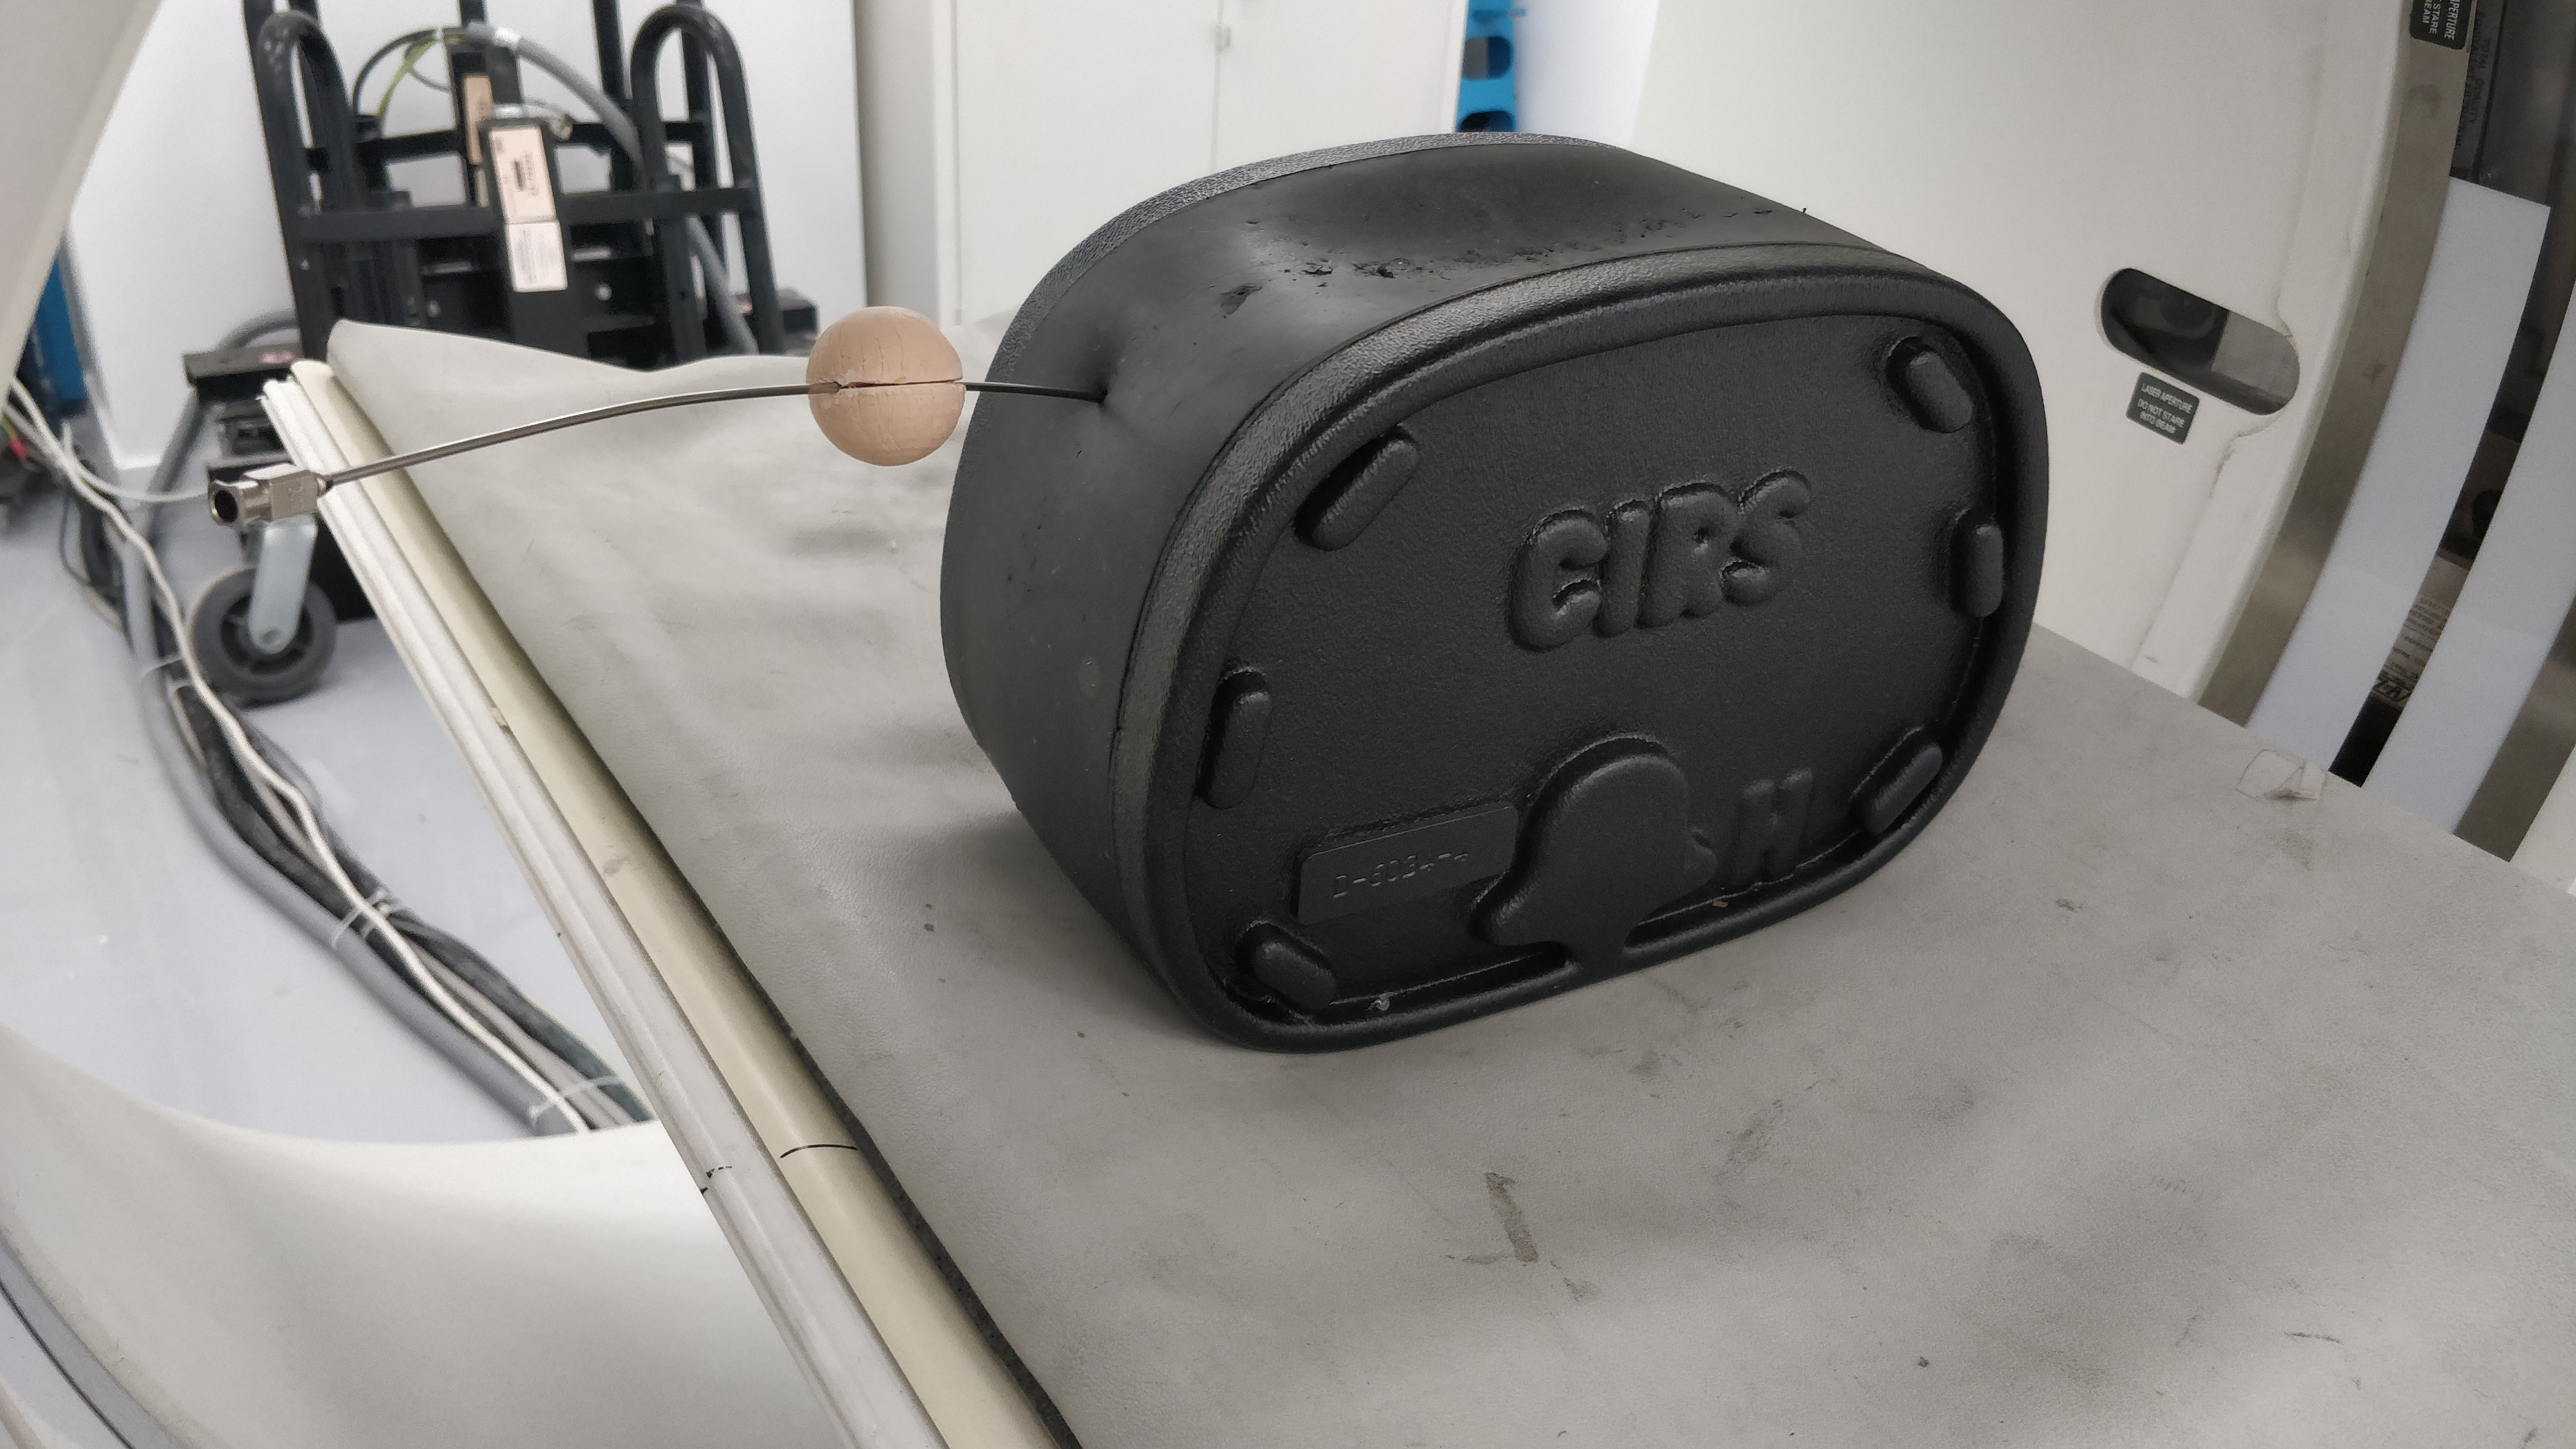
\includegraphics[width=0.45\textwidth]{long_needle_phantom.jpg}
  \label{long_needle_fig}}
  \hfill
  \subfloat[]{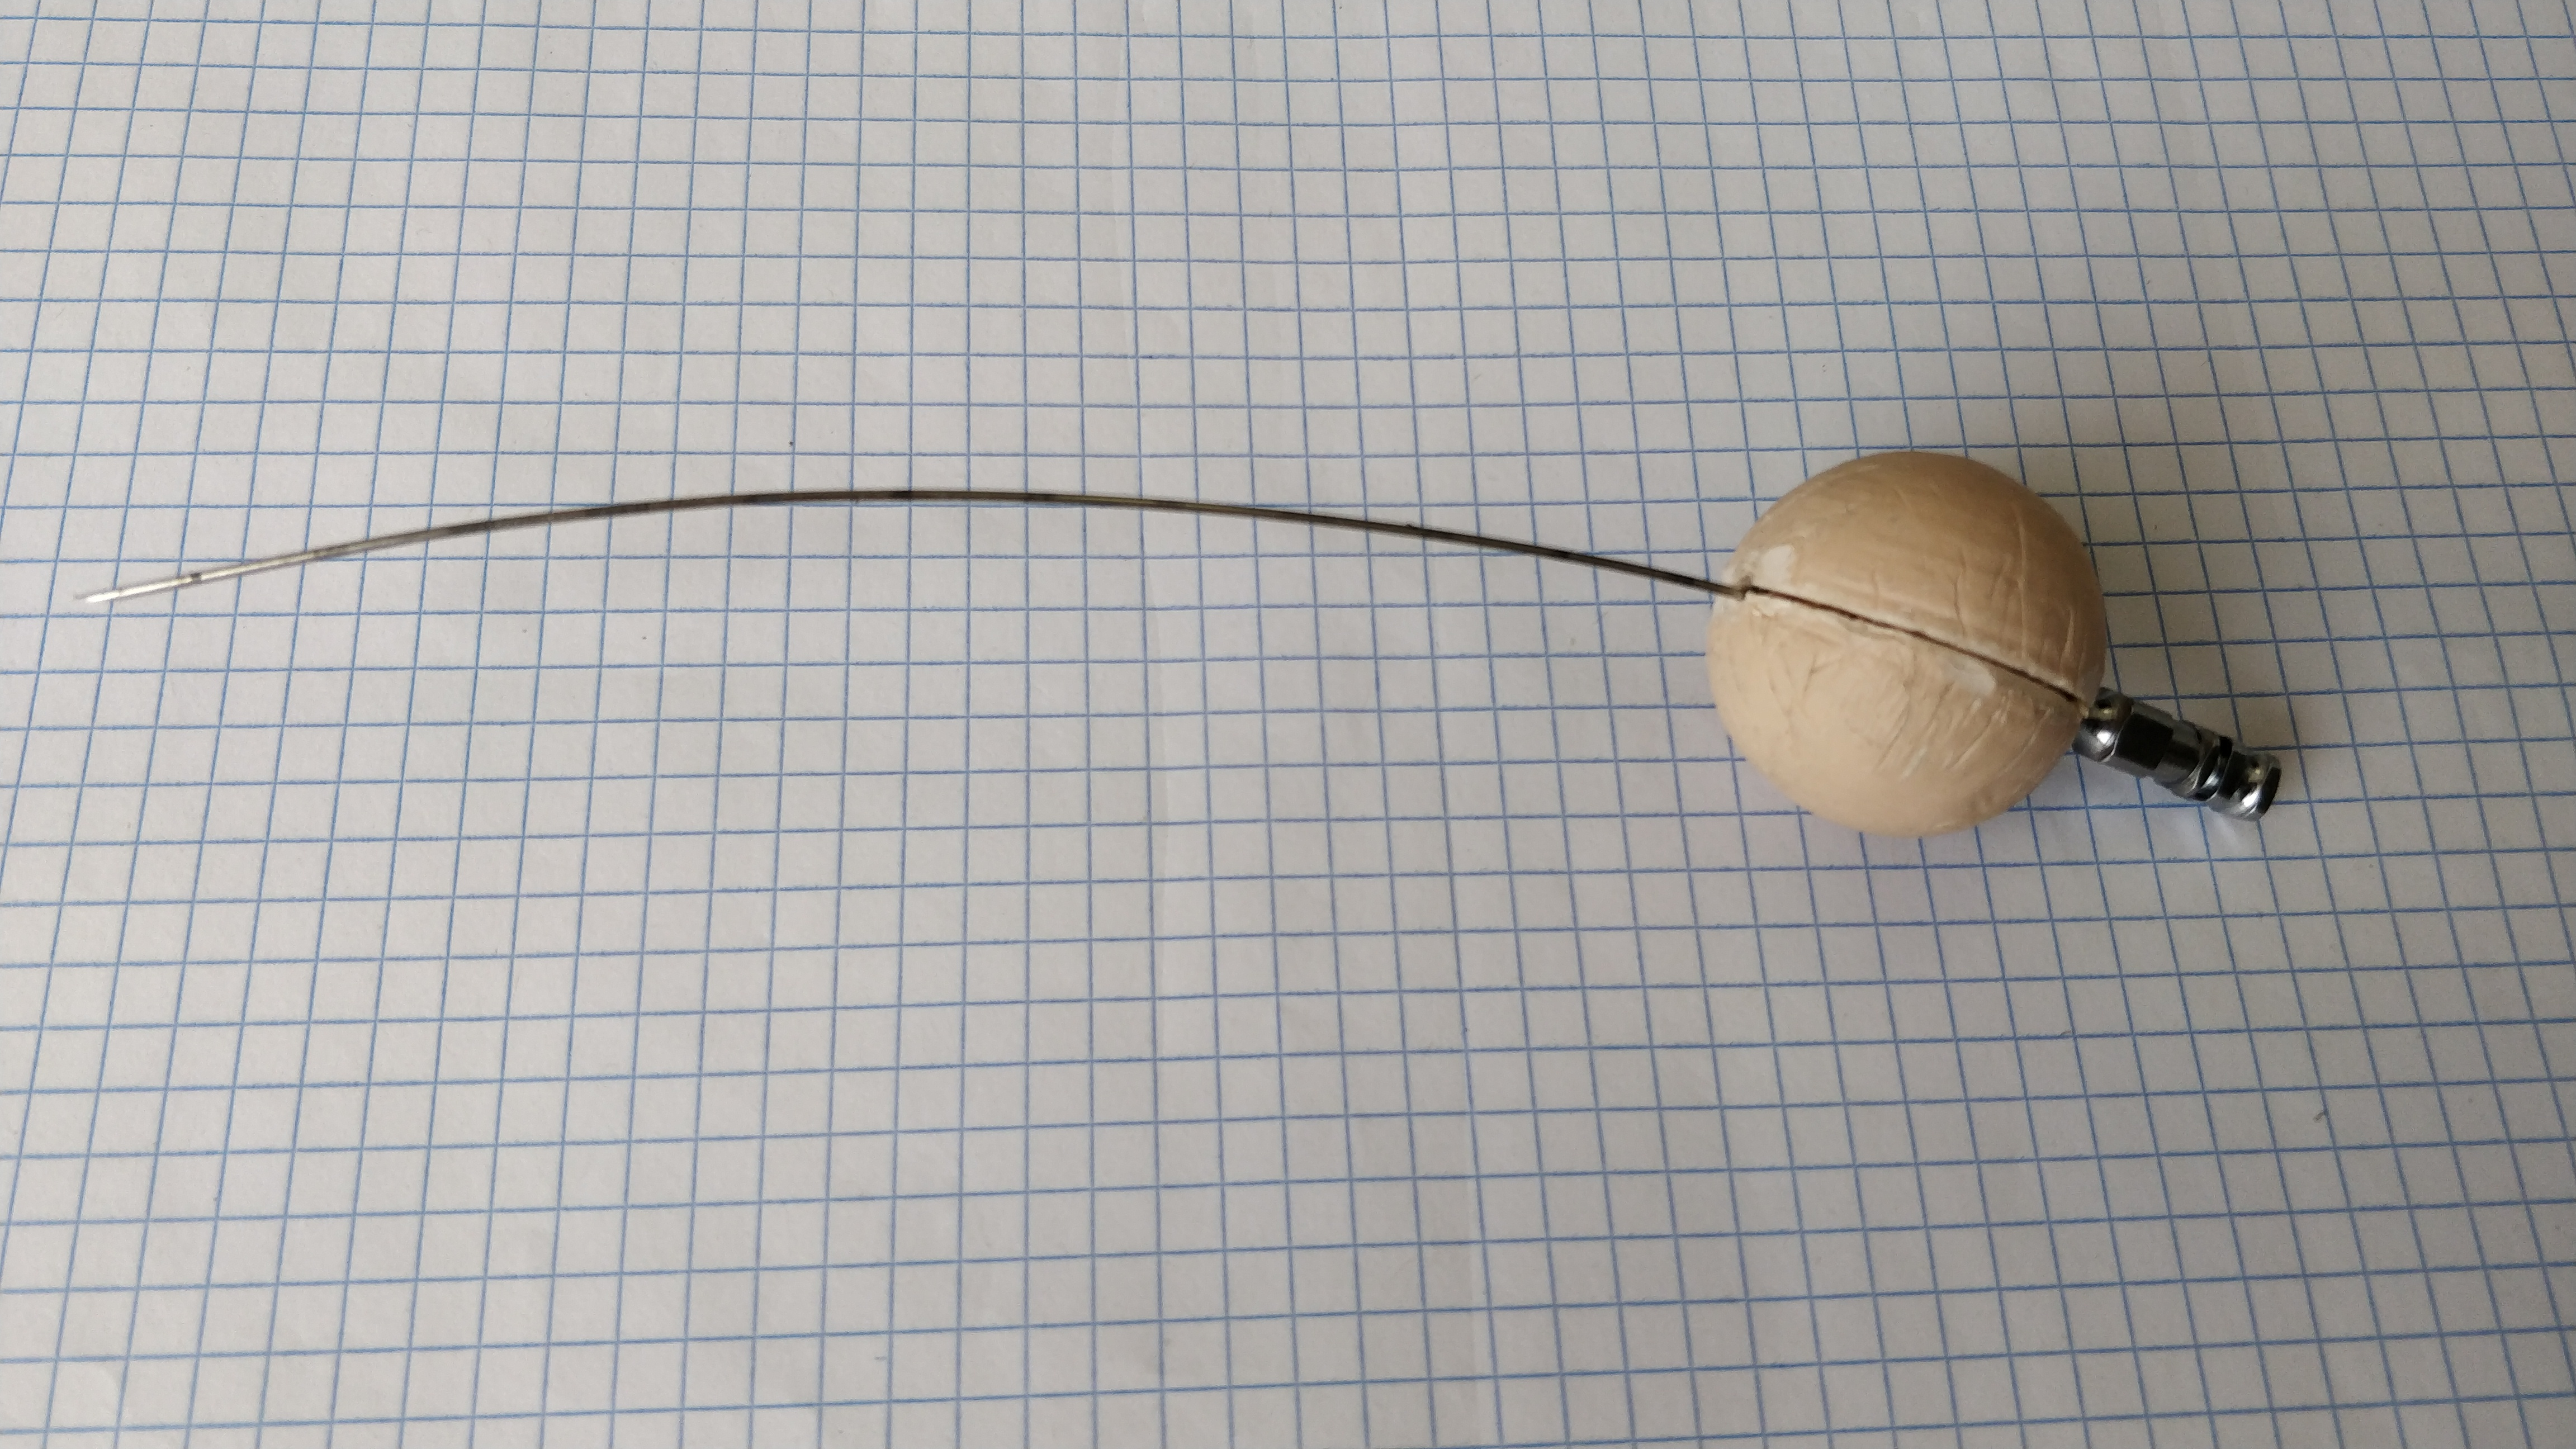
\includegraphics[width=0.45\textwidth]{short_needle.jpg}
  \label{short_needle_fig}}
  \caption{\small{Experimental setup for flexible needle insertion with abdomen phantom. (a) Photograph of the long flexible needle with spherical marker inserted into abdomen phantom lying on the CT scanner bed. (b) Photograph of the short flexible needle with spherical marker attached at 135mm from the tip.}}
    \label{fig:figures/fractional}
\end{figure*}


\begin{table}[t]
\begin{center}
\begin{tabular}{|c||c|c|c|c|}
\hline
Scan & Reg. error & Marker & Tip error & Trajectory\\
ID  & [mm] & error [mm] & [mm] & error  [mm]\\
\hline
\hline
L1 & 1.4 & 1.9 & 2.6 & 0.7\\
\hline
L2 & 0.7 & 0.8 & 1.9 & 0.6\\
\hline
L3 & 0.6 & 0.3 & 4.3 & 0.9 \\
\hline
L4 & 1.0 & 0.8 & 2.0 & 0.5\\
\hline
S1 & 1.4 & 1.1 & 2.4 & 0.5\\
\hline
S2 & 1.2 & 1.5 & 1.4 & 0.6\\
\hline
S3 & 1.5 & 0.9 & 2.2 & 0.9\\
\hline
\hline
L & 
0.9 $\pm\hspace{0.04cm}$ 0.4 & 
1.0 $\pm\hspace{0.04cm}$ 0.7 & 
2.7 $\pm\hspace{0.04cm}$ 1.1 & 
0.7 $\pm\hspace{0.04cm}$ 0.2\\
\hline
S & 
1.4 $\pm\hspace{0.04cm}$ 0.2 &  
1.2 $\pm\hspace{0.04cm}$ 0.3 & 
2.0 $\pm\hspace{0.04cm}$ 0.5 &  
0.7 $\pm\hspace{0.04cm}$ 0.2\\
\hline
ALL & 
1.1 $\pm\hspace{0.04cm}$ 0.4 &  
1.0 $\pm\hspace{0.04cm}$ 0.5 &  
2.4 $\pm\hspace{0.04cm}$ 0.9 &  
0.7 $\pm\hspace{0.04cm}$ 0.2\\
\hline
\end{tabular}
\caption{\small{Summary of experimental results. L/S stands for long/short needle, respectively.
The bottom part of the table shows means and standard deviations across the long, short and all scans in the dataset.}}
\label{results_table}
\end{center}
\end{table}





\begin{figure}[b]
\centering
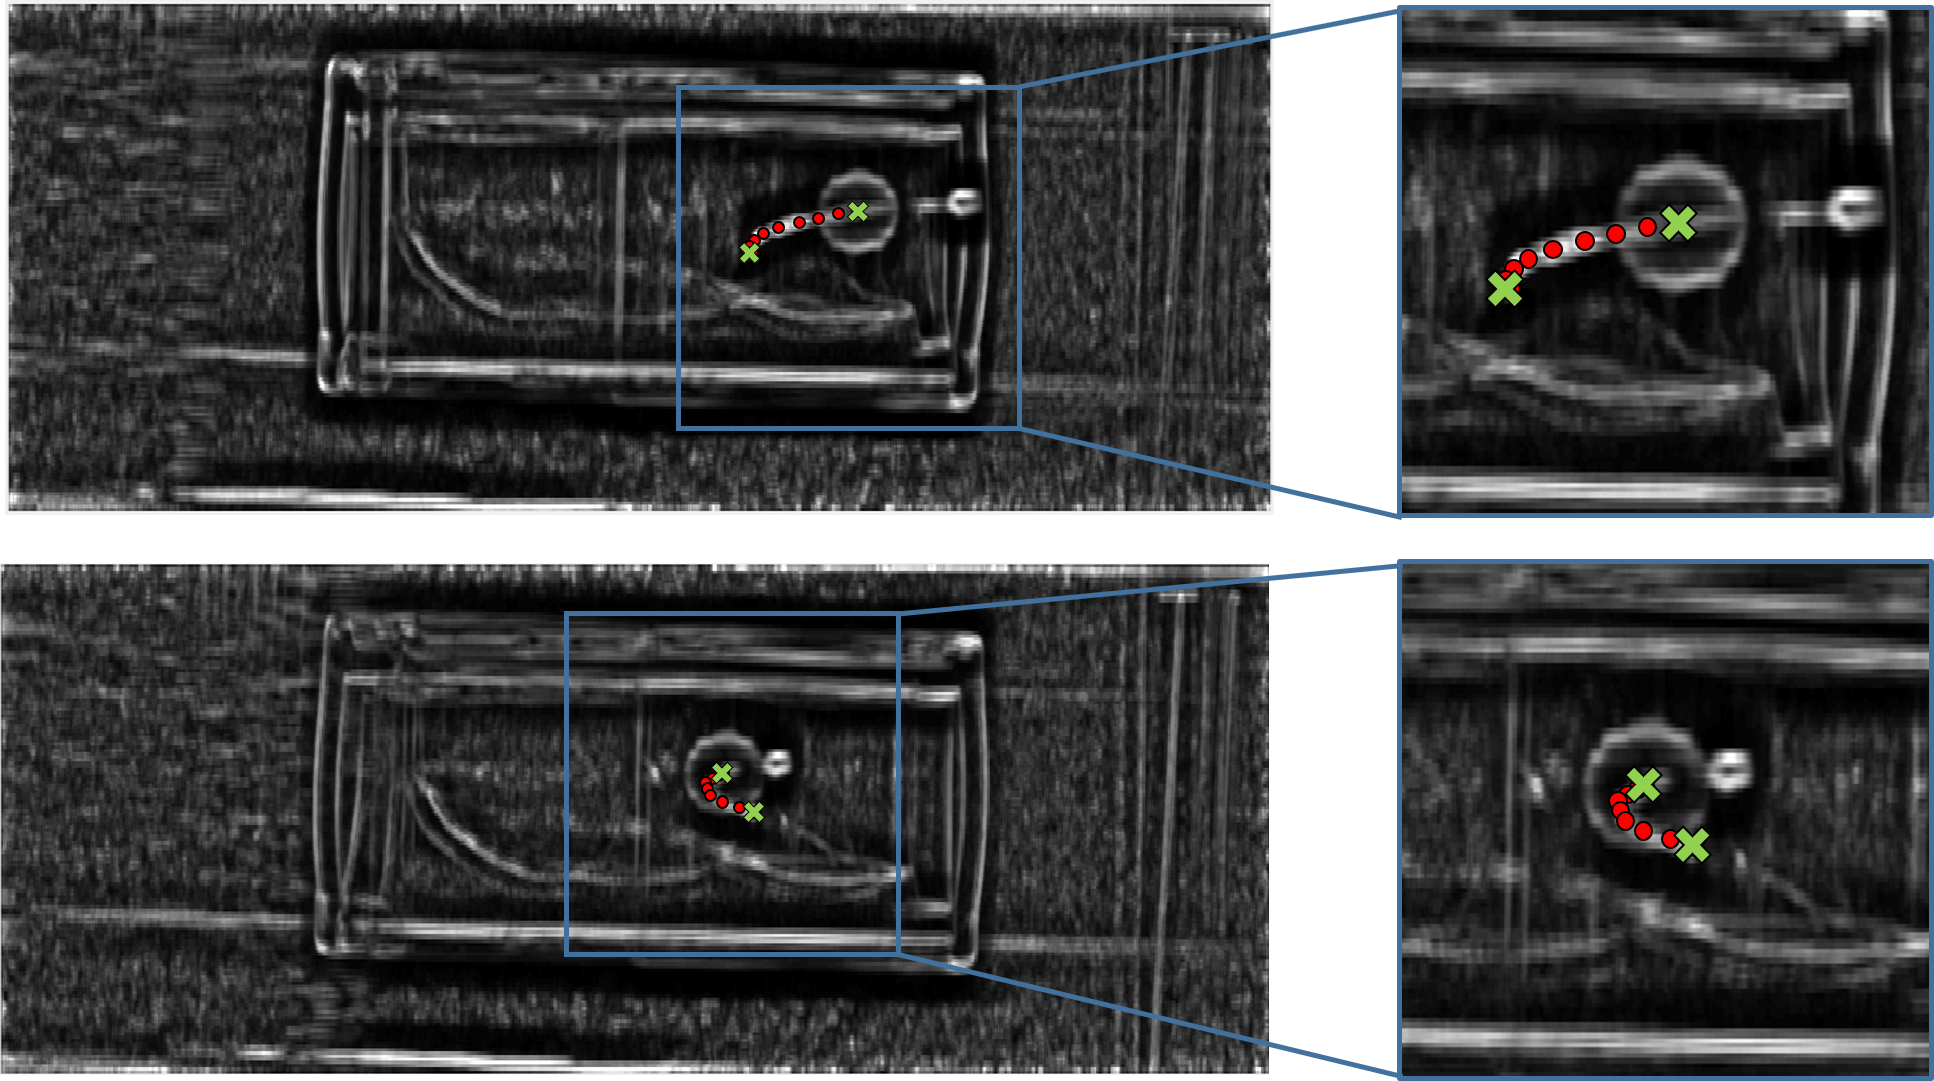
\includegraphics[width=\textwidth]{projection_diff_images.png}
\caption{\small{Projection difference images for two views from one scan of the short needle (left), and zoom in on the needle in each image (right). the green crosses indicate ground truth center of marker and tip; red dots indicate the landmark points established in the incremental needle trajectory fitting.}}
\label{proj_diff_fig}
\end{figure}

The full baseline scan was registered to each sparse scan with needle inserted, using Radon-space rigid registration. The registration accuracy was evaluated as the root-mean-square of differences between voxel coordinates transformed by the calculated registration and by image-space registration of the reconstructed images. 
A sparse set of 24 evenly spaced view angles in the range [0$^\circ$,180$^\circ$) was used for Radon-space registration and needle trajectory fitting as previous experiments \cite{medan2017reduced} with a straight needle showed this selection offered a good trade-off between robustness and potential dose reduction. The segment length parameter $\Gamma$ was set to 15mm, as experimentation showed that shorter values were not as resilient to feature noise in the optimization of segments directions, and longer values overshoot the typical bending of the needles in the experiments.
The marker center ground truth was obtained via manual localization on the reconstructed images, and the trajectory ground truth was traced in 3D image space manually by placing landmark points based on a volumetric difference image, and cubic B\'ezier curve fitting in 3D. The tip ground truth was determined as the point on the needle trace found at the known tip-marker distance. The trajectory error was evaluated as the root-mean-squared distance of points along the fitted curve to the nearest point on the ground-truth curve.

Table \ref{results_table} summarizes the results of needle tip localization for the 7 scans in the dataset. One of the scans (L3) shows a large tip localization error due to the needle trajectory being very close to in-plane with the axial plane (see Fig. \ref{multislices_fig}). In our method, long needle segments that are in-plane lead to inaccurate estimation of the trajectory since the projections of such segments are observed as horizontal lines in the projection difference images regardless of the orientation within the plane. This imposes a limitation encountered previously in our work on straight needles \cite{medan2017reduced}, where in-plane insertion of the needle should be avoided to enable the recovery of the needle orientation as an intersection of non-parallel planes.

Running times of 200-250 seconds were observed on Intel i7 CPU running unoptimized Matlab code. To allow our method to be used in a clinical setting, parallelization of computations on GPU will be required in order to bring the running time down to several seconds. In the projection difference calculation stage, the projection difference images can be calculated in parallel. Additionally, in each round of landmark point addition, the operations on each projection difference image can be parallelized to further reduce the running time.

\section*{Discussion}
Our method extends the novelty of projection-space localization from rigid to flexible needles, allowing the potential of dose reduction in a larger range of interventional CT procedures. The localization can be displayed as visual feedback to the radiologist on the baseline scan, which is free from artifacts due to the needle, allowing an unobstructed view of the target tissue.

\begin{figure*}
\centering
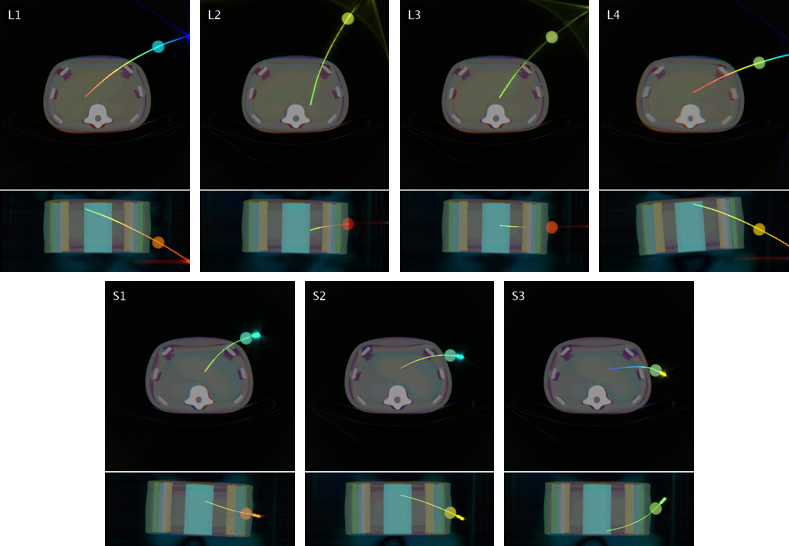
\includegraphics[width=\textwidth]{multislices.png}
\caption{\small{Axial and coronal multi-slice views (top and bottom of each sub-image, respectively) of the abdomen phantom with flexible needle (L-long, S-short) inserted in different positions. The multi-slice views are generated by assigning a color map to encode the depth of each slice in the direction perpendicular to the image plane.}}
\label{multislices_fig}
\end{figure*}

The quantitative feedback enabled by our approach is particularly important for robotically driven needles, where the interaction of the needle and tissue is modeled in order to construct a control sequence realizing a planned insertion path. Such systems would benefit from mid-insertion feedback that would allow adjustments to the control sequence based on the achieved state of the needle insertion, and a reduction in X-ray dose will benefit the patient who will be subjected to a smaller radiation-related risk.


Our method is suitable when the baseline and repeat scans have minimal deformations and rigid registration can be used to align them. The scan field of view needs to includes the flexible needle and the spherical marker, while keeping the insertion out-of-plane. The spherical marker is unintrusive to the intervention workflow in the sense that it only requires pre-attachment to the needle by medical staff and does not obstruct the interventionalist's routine.

The study itself is limited to several scans of an abdomen phantom, with the fractional scanning simulated from full scans by omitting most of the repeat scan data used as input for the algorithm. To implement our method on a commercial CT scanner, fractional scanning would have to be achieved by one of two possible approaches: fast modulation of the X-ray tube current and/or voltage, or fast mechanical collimation during acquisition. Such methods would require hardware integration beyond the scope of this work, but since the fraction of views required in the repeat scan is below 5\%, there is potential for substantial dose reduction.

Future work would address the issue of patient motion during the repeat scan to obtain a better localization of the needle by modelling the movement and finding its parameters directly from projection space. Additionally, deformable registration in projection space as another stage after rigid registration would extend the usability of our method to situations in which tissue deformations, such as those caused by breathing, cannot be neglected.

\section*{Conclusions}
We have described a method for flexible needle and patient tracking in interventional CT procedures, based on fractional CT scanning and without image reconstruction of the repeat scan.
Our method can accurately trace a flexible needle's 3D trajectory by following its shape in projection space for a sparse set of views. Starting from a spherical marker attached to it at a known distance from the tip, it traces the trajectory to the tip without reconstructing the CT image.

The main advantages of our method are:
1) accurate flexible needle trajectory and needle tip localization without image reconstruction;
2) significant potential dose reduction for each individual repeat scan localization;
3) simultaneous patient registration and needle localization for every snapshot; 
4) fully automatic, no calibration and/or manual setup;
5) only a simple marker attached to the needle is required; 
6) artifact-free monitoring of a flexible needle's trajectory on top of a baseline scan.

In a limited phantom study performed in cooperation with a leading CT manufacturer, an accuracy level comparable to 3D image space methods is shown.
The dose reduction enabled by our method allows either more frequent tip localizations during needle insertion for a similar total dose, or a reduced total dose for the same frequency of tip localization - a reduction of $\times$10-25, based on the fraction of views used from the repeat scan.

\bibliographystyle{spbasic_order_of_appearance}
\bibliography{flexible_needle}

\end{document}
% end of file template.tex

